% !TeX program = xelatex
\documentclass[11pt,a4paper]{ctexart}
\usepackage[margin=2.3cm]{geometry}
\usepackage{booktabs}
\usepackage{float}
\usepackage{graphicx}
\usepackage{xcolor}
\usepackage{tikz}
\usetikzlibrary{arrows.meta,positioning,shapes.geometric,fit,backgrounds}
\usepackage[margin=1.1cm,font=small,labelfont=bf]{caption}
\usepackage[hidelinks]{hyperref}

\definecolor{cblue}{HTML}{1C7ED6}
\definecolor{cgreen}{HTML}{2B8A3E}
\definecolor{corange}{HTML}{F08C00}
\definecolor{cred}{HTML}{C92A2A}
\definecolor{cgray}{HTML}{495057}

\begin{document}

\begin{titlepage}
\centering
\vspace*{2.2cm}
{\Huge\bfseries 机器人控制策略优化算法对比\\[0.5em] 正式实验报告\par}
\vspace{0.9cm}
{\Large Reinforcement-Learning-Policy · v2 机器人控制套件\par}
\vspace{0.5cm}
{\large 12 算法 $\times$ 3 任务 $\times$ 4 奖励范式 $\times$ 3 种子 = 189 组受控实验\par}
\vspace{2.2cm}
{\large\itshape 同步自仓库 README\_CN.md(v2.1,2026-11-14)\par}
\vspace{2.6cm}
\begin{tabular}{rl}
\textbf{作 者} & Aitachi\\
\textbf{联 系} & 44158892@qq.com\\
\textbf{仓 库} & \url{https://github.com/aitachi/Reinforcement-Learning-Policy}\\
\textbf{许 可} & MIT\\
\textbf{日 期} & 2026 年 11 月 14 日\\
\end{tabular}
\vfill
\end{titlepage}

\tableofcontents
\newpage

\section*{摘要}
本报告是 \textbf{Reinforcement-Learning-Policy} 仓库 v2 机器人控制套件的正式实验报告,内容与仓库双语 README 完全同步。套件在统一公平性协议(相同采样预算、网络规模、优化器与种子)下,对 \textbf{12 种}策略优化算法——信赖域近端家族(PPO-Clip/KL/RB/TR-RB/ESPO、PPG、TRPO、A2C)、源自 LLM 后训练的组相对家族(GRPO-C、DAPO-C)与异策略锚点(SAC、TD3)——在 3 个自包含机器人任务(E1 避障导航、E2 单足运控、E3 抓取-提起)上展开对比,每个任务配备稀疏/稠密/势函数(PBS)/课程四种奖励范式,共计 \textbf{189 组}受控实验,并产出两篇 IEEE 论文与本报告。报告除汇总核心结果表外,提供训练循环与产线管线两张矢量流程图、算法知识图谱,以及算法$\times$任务、奖励范式$\times$算法$\times$任务两幅三维对比图。核心结论:信赖域保险(自适应 KL/早停/信赖域回滚)决定接触密集任务的可靠性;TRPO 在 E3 取得种子满分 1.000;SAC 以 5--8$\times$ 墙钟代价取得 E1+E2 双冠;组相对方法仅在 outcome 型任务可用;奖励范式与算法必须联合选择。

\section{项目背景与双轨道架构}

本仓库包含\textbf{两条物理隔离的研究轨道},共享同一研究问题——\emph{在受控、预算对齐的条件下,信赖域近端家族与组相对家族各自表现如何?结论又如何随奖励信号改变?}

\begin{table}[H]
\centering
\caption{双轨道导航}
\small
\begin{tabular}{l l p{4.6cm} p{4.4cm}}
\toprule
轨道 & 状态 & 领域与规模 & 入口 \\
\midrule
\textbf{v2 机器人控制} & 当前版本 & 12 算法 $\times$ 3 任务 $\times$ 4 范式,189 组,2 篇论文 & \texttt{control/} \texttt{papers/} \texttt{results/} \\
v1 LLM 后训练 & 原版冻结 & Qwen2-1.5B 上的 PPO/DPO/GRPO/DAPO + IEEE 综述 & \texttt{v1-llm-post-training/} \\
\bottomrule
\end{tabular}
\end{table}

本报告对应 \textbf{v2 轨道};v1 轨道另有约 600 行/语言的完整文档(中/英/日),不在本报告范围内。

\section{实验设置}

\subsection{任务环境(E1--E3)}

三个任务均为纯 PyTorch、GPU 批量化实现(64--128 并行回合),不依赖 MuJoCo 等外部物理引擎;任务信号与奖励范式解耦,任意奖励可驱动任意任务。

\begin{table}[H]
\centering
\caption{任务环境一览(中等难度标定:2 层 MLP 可在 $\le$600k 步内求解)}
\small
\begin{tabular}{l p{4.5cm} c c p{3.1cm} c}
\toprule
任务 & 机制 & 观测/动作 & 回合长 & 成功判据 & 总步数 \\
\midrule
E1 \texttt{nav} & 全向机器人穿越随机障碍场(8 线激光雷达) & 14 / 2 & 150 & 到达目标($\le$0.06),碰撞即败 & 400k \\
E2 \texttt{hopper} & 5-DOF 平面单足,串联弹性膝关节($k{=}18$) & 14 / 2 & 250 & 位移 3\,m 不摔倒 & 600k \\
E3 \texttt{grasp} & 速度控制三连杆臂,滞回抓取 & 16 / 4 & 160 & 持举物体 15\,cm & 500k \\
\bottomrule
\end{tabular}
\end{table}

\subsection{算法(12 种)}

\begin{table}[H]
\centering
\caption{算法家族划分}
\begin{tabular}{l p{10.8cm}}
\toprule
家族 & 算法 \\
\midrule
PPO 近端家族(方法开关) & PPO-Clip、PPO-KL(自适应)、PPO-RB(回滚)、TR-PPO-RB(信赖域回滚)、ESPO(早停) \\
阶段化 / 经典同策略 & PPG、TRPO(CG + 回溯线搜)、A2C \\
组相对(源自 LLM RL) & GRPO-C、DAPO-C(回合结果基线、clip-higher、动态采样、超时过滤) \\
异策略锚点 & SAC、TD3 \\
\bottomrule
\end{tabular}
\end{table}

\subsection{奖励范式与公平性协议}

每个任务配备 \textbf{sparse / dense / PBS(势函数)/ curriculum} 四种范式,合计 12 个带逐项审计的奖励函数;每个奖励项在训练时全程记录(奖励黑客遥测,论文 2 含抓取边界抖动刷奖的完整案例研究)。

\textbf{公平性协议:}统一采样(64 环境 $\times$ 256 步 rollout)、$2\times128$ tanh MLP 正交初始化、Adam $3\times10^{-4}$(TRPO 主角 $3\times10^{-5}$;GRPO/DAPO $10^{-4}$)、梯度范数裁剪 0.5、GAE $(0.99,0.95)$、价值裁剪、4 内层 epoch、minibatch 2048;每 20k 步以确定性策略在 64 个满难度 held-out 回合上评估。

\textbf{实验网格:}A 轴(算法)12 算法 $\times$ 3 任务 $\times$ 3 种子,dense 奖励(108 组);B 轴(奖励)其余 3 范式 $\times$ 3 任务 $\times$ 3 种子 $\times$ 3 代表算法(PPO-Clip、TRPO、GRPO-C,与 A 轴共享 dense)(81 组),合计 \textbf{189 组}。

\section{实验工作流}

\subsection{单回合训练循环}

\begin{figure}[H]
\centering
\begin{tikzpicture}[
  node distance=7mm and 9mm,
  box/.style={draw=cgray,rounded corners=2pt,align=center,inner sep=6pt,font=\small,fill=white,thick},
  io/.style={box,fill=black!4},
  dec/.style={box,fill=black!4},
  fl/.style={-{Stealth[length=2.4mm]},thick,cgray},
  lbl/.style={font=\scriptsize,cgray}]
\node[box,fill=cblue!12] (collect) {\textbf{向量化采集}\\64 环境 $\times$ 256 步};
\node[box,right=of collect] (gae) {\textbf{GAE 优势估计}\\$\gamma{=}0.99,\ \lambda{=}0.95$};
\node[box,right=of gae,fill=cgreen!12] (update) {\textbf{策略更新(方法开关)}\\近端:Clip / KL / RB / TR-RB / ESPO\\阶段化:PPG / TRPO / A2C\\组相对:GRPO-C / DAPO-C\\异策略:SAC / TD3};
\node[box,below=of update,fill=corange!14] (eval) {\textbf{确定性评估}\\64 held-out 回合\\每 20k 步};
\node[io,below=of collect] (log) {CSV 学习曲线\\JSON 汇总};
\node[io,below=of gae] (audit) {\textbf{奖励逐项审计}\\每项均值全程记录};
\draw[fl] (collect) -- (gae);
\draw[fl] (gae) -- (update);
\draw[fl] (update) -- (eval);
\draw[fl] (eval.west) -| node[lbl,pos=0.22,above]{下一迭代} ([xshift=-6mm]collect.south west) |- (collect.west);
\draw[fl] (eval.south) -- ++(0,-4.5mm) -| node[lbl,pos=0.25,below]{终值输出} (log.south);
\draw[fl] (gae) -- (audit);
\end{tikzpicture}
\caption{单回合训练循环:采集 $\to$ GAE $\to$ 策略更新 $\to$ 确定性评估,输出曲线与奖励审计。}
\end{figure}

\subsection{全量产线管线}

\begin{figure}[H]
\centering
\begin{tikzpicture}[
  node distance=6mm and 8mm,
  stage/.style={draw=cgray,rounded corners=2pt,align=center,inner sep=6pt,font=\small,thick},
  fl/.style={-{Stealth[length=2.4mm]},thick,cgray}]
\node[stage,fill=cblue!12] (train) {\texttt{train.py}\\统一训练入口\\{\scriptsize --env --algo --reward --seed}};
\node[stage,right=of train,fill=cblue!12] (sweep) {\texttt{sweep.py}\\全网格 189 组\\{\scriptsize 可断点续跑 (catchup.py)}};
\node[stage,right=of sweep,fill=cgreen!12] (ana) {\texttt{analysis.py}\\出版级图 + \texttt{.tex} 表\\{\scriptsize results/figs/}};
\node[stage,below=of ana,fill=cgreen!12] (gen) {\texttt{gen\_results.py}\\headline.json + findings};
\node[stage,below=of sweep,fill=corange!14] (papers) {论文 1(算法对比)\\论文 2(奖励设计)\\{\scriptsize IEEEtran,build\_papers.bat}};
\node[stage,below=of train,fill=corange!14] (report) {本实验报告\\{\scriptsize XeLaTeX + TikZ}};
\node[stage,left=of report,fill=black!5] (git) {REST API 同步\\github.com};
\draw[fl] (train) -- (sweep);
\draw[fl] (sweep) -- (ana);
\draw[fl] (ana) -- (gen);
\draw[fl] (sweep) -- (papers);
\draw[fl] (papers) -- (report);
\draw[fl] (report) -- (git);
\end{tikzpicture}
\caption{产线管线:单次训练 $\to$ 全网格 $\to$ 分析/汇总 $\to$ 论文与本报告,数据一次生成、处处复用。}
\end{figure}

\section{核心结果}

\subsection{总表(dense 奖励,3 种子均值,189 组)}

\begin{table}[H]
\centering
\caption{12 算法 $\times$ 3 任务核心结果(与 README\_CN 完全同步)}
\begin{tabular}{lcccl}
\toprule
算法 & E1 导航成功率 & E2 单足位移 & E3 抓取提起 & 备注 \\
\midrule
SAC & \textbf{0.830} & \textbf{0.899} & 0.629 & 慢 5--8$\times$(E2 4403\,s) \\
PPG & 0.673 & 0.020 & 0.998 & E1 仅 39\,s \\
TRPO & 0.669$\pm$0.02 & 0.681 & \textbf{1.000$\pm$0.00} & CG + 线搜开销 \\
PPO-KL & 0.658 & 0.785 & 0.992 & \\
PPO-RB & 0.655 & 0.669 & 0.995 & \\
PPO-Clip & 0.652 & 0.620 & 0.996 & E2 种子散布 $\pm$0.17 \\
ESPO & 0.648 & 0.755 & 0.568 & \\
TR-PPO-RB & 0.625 & 0.754 & 0.694 & \\
GRPO-C & 0.557$\pm$0.07 & 0.017 & 0.000 & 仅 E1 中游 \\
A2C & 0.547 & 0.027 & 0.059 & \\
TD3 & 0.434 & 0.167 & 0.000 & 种子彩票 \\
DAPO-C & 0.324 & 0.015 & 0.000 & \\
\bottomrule
\end{tabular}
\end{table}

\begin{figure}[H]
\centering
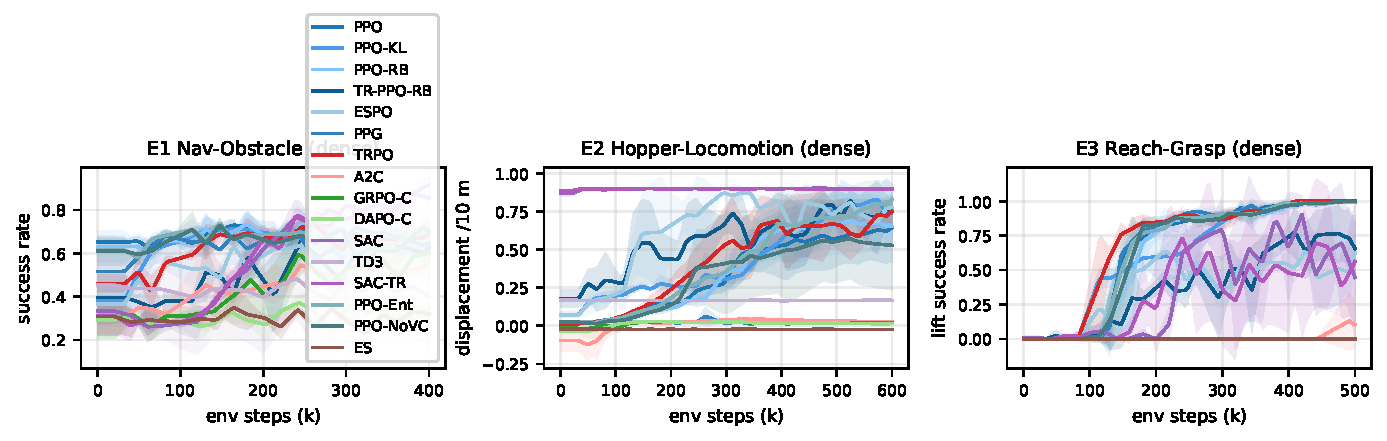
\includegraphics[width=\textwidth]{../../results/figs/curves_dense.pdf}
\caption{dense 奖励学习曲线(3 种子均值 $\pm$95\% CI,每 20k 步确定性评估;左 E1 成功率 / 中 E2 位移 / 右 E3 提起率)。}
\end{figure}

\begin{figure}[H]
\centering
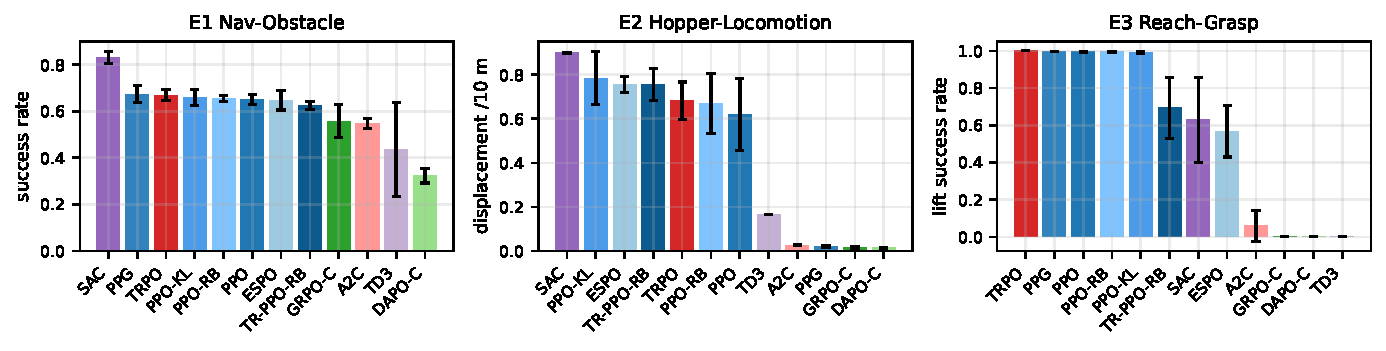
\includegraphics[width=0.86\textwidth]{../../results/figs/final_bars_dense.pdf}
\caption{dense 终值柱状对比(末 5 次评估均值 $\pm$ 标准差,3 种子)。}
\end{figure}

\subsection{三维对比}

\begin{figure}[H]
\centering
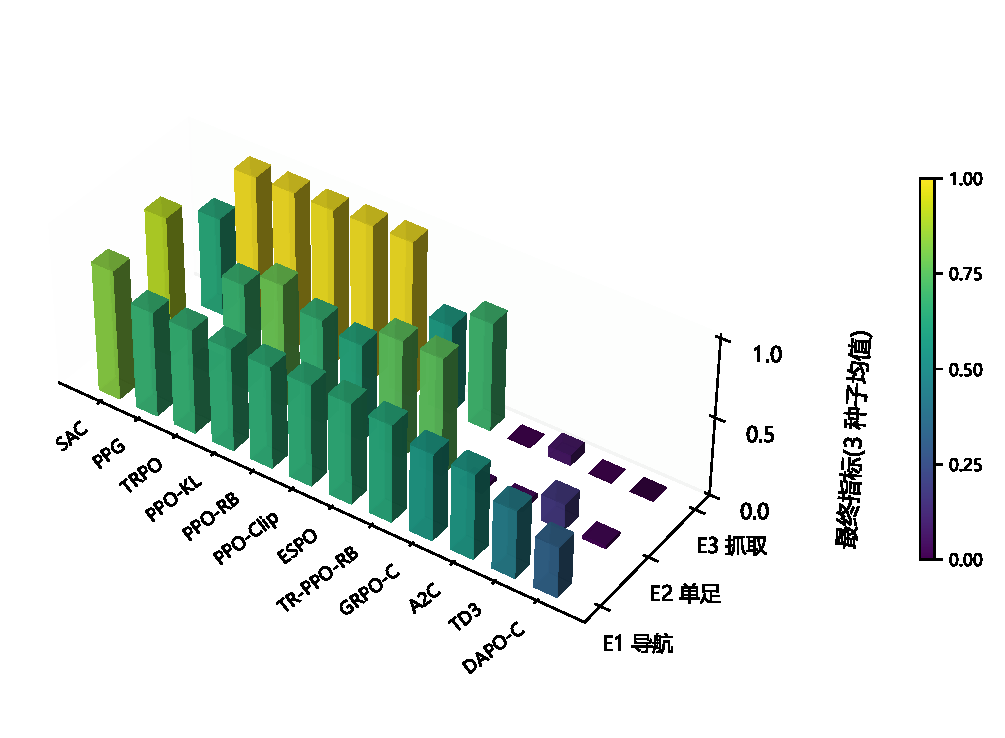
\includegraphics[width=0.94\textwidth]{figs/fig3d_algo_task.pdf}
\caption{算法 $\times$ 任务三维对比(12 $\times$ 3 根柱,颜色即数值)。E1 前排:SAC 一枝独秀;E2 中排:SAC 领跑、PPO 家族靠保险上位、GRPO-C/DAPO-C 与 A2C/PPG 塌底;E3 后排:TRPO 满分 1.000、PPO 家族全员 $\ge$0.99、TD3/GRPO-C/DAPO-C 归零。}
\end{figure}

\begin{figure}[H]
\centering
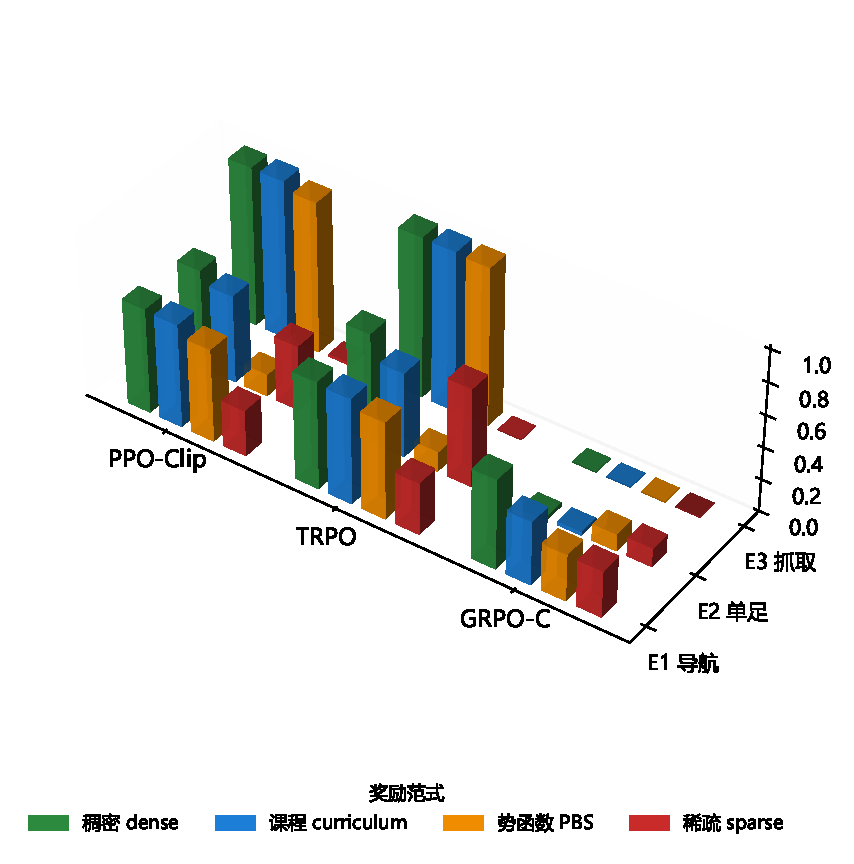
\includegraphics[width=0.94\textwidth]{figs/fig3d_paradigm.pdf}
\caption{奖励范式 $\times$ 算法 $\times$ 任务三维对比(B 轴 108 组)。可见 PBS 在 E2 对 PPO/TRPO 的塌方(约 0.12)、GRPO-C 在 E2 的 sparse$>$dense 反转,以及 E3 全系 sparse 归零。}
\end{figure}

\subsection{奖励轴明细}

\begin{table}[H]
\centering
\caption{奖励范式 $\times$ 算法 $\times$ 任务终值(3 种子均值)}
\begin{tabular}{llcccc}
\toprule
任务 & 算法 & 稀疏 sparse & 稠密 dense & 势函数 PBS & 课程 curriculum \\
\midrule
E1 导航 & PPO-Clip & 0.286 & 0.652 & 0.577 & 0.643 \\
E1 导航 & TRPO & 0.323 & 0.669 & 0.604 & 0.656 \\
E1 导航 & GRPO-C & 0.288 & 0.557 & 0.290 & 0.395 \\
\midrule
E2 单足 & PPO-Clip & 0.407 & 0.620 & \textcolor{cred}{0.133} & 0.546 \\
E2 单足 & TRPO & 0.612 & 0.681 & \textcolor{cred}{0.120} & 0.526 \\
E2 单足 & GRPO-C & \textbf{0.109} & 0.017 & 0.097 & 0.016 \\
\midrule
E3 抓取 & PPO-Clip & \textcolor{cred}{0.009} & 0.996 & 0.944 & 0.993 \\
E3 抓取 & TRPO & \textcolor{cred}{0.000} & \textbf{1.000} & 0.984 & 0.996 \\
E3 抓取 & GRPO-C & 0.000 & 0.000 & 0.000 & 0.000 \\
\bottomrule
\end{tabular}
\end{table}

\begin{figure}[H]
\centering
\begin{minipage}{0.44\textwidth}
\centering
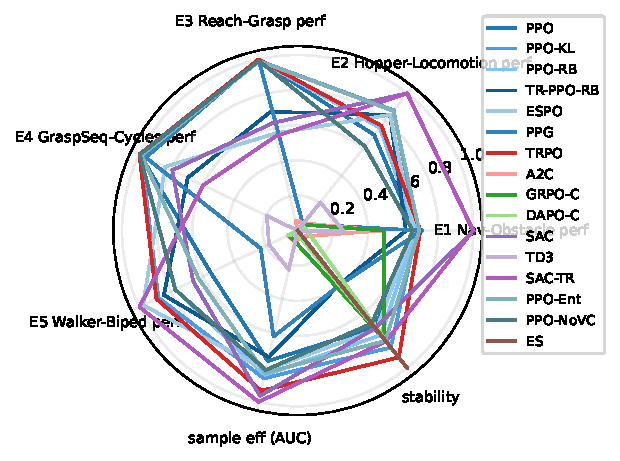
\includegraphics[width=\textwidth]{../../results/figs/radar.pdf}
\end{minipage}\hfill
\begin{minipage}{0.54\textwidth}
\centering
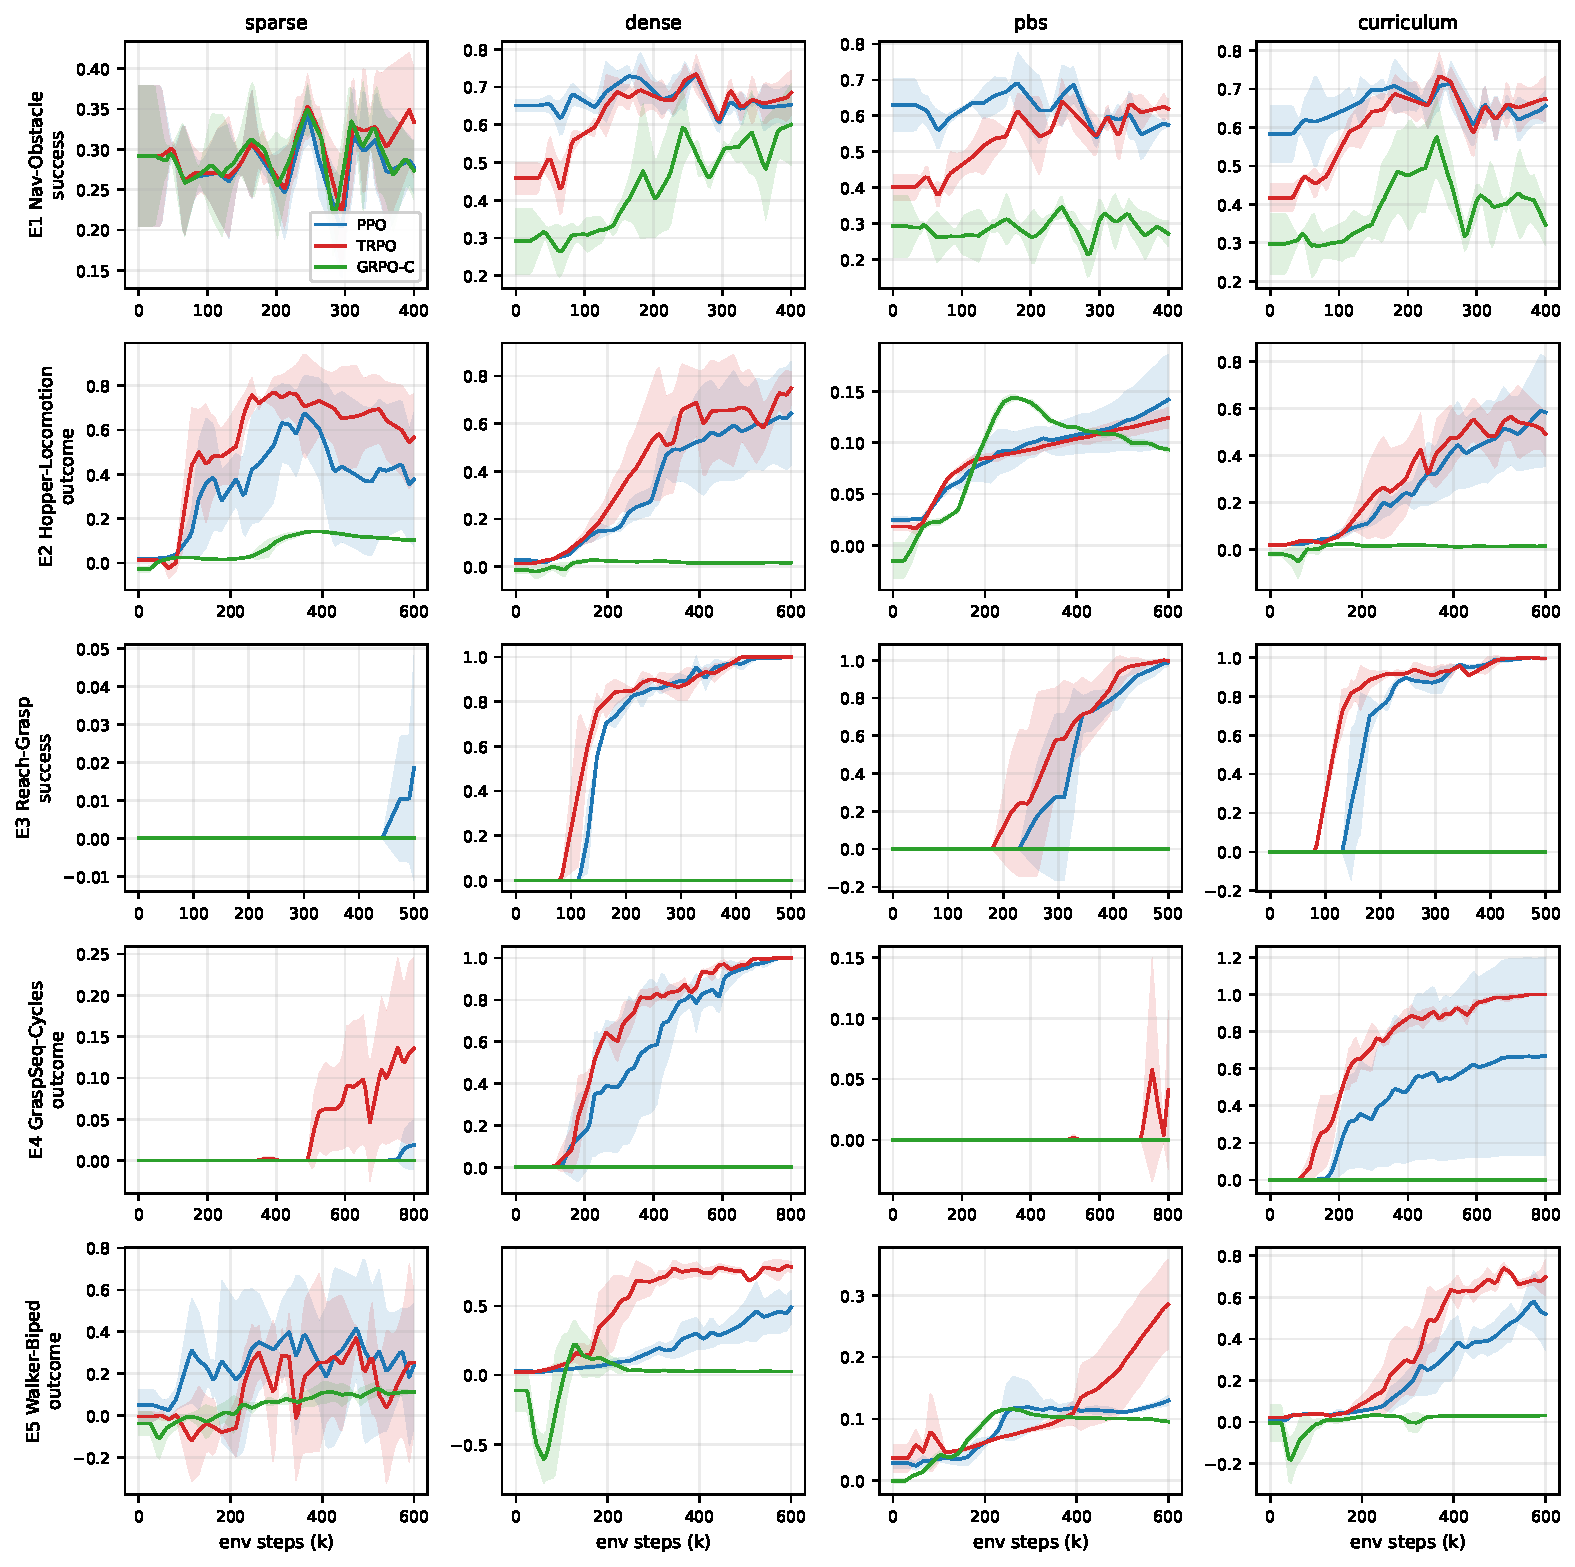
\includegraphics[width=\textwidth]{../../results/figs/reward_paradigm_grid.pdf}
\end{minipage}
\caption{左:归一化多维画像(终值 / 样本效率 AUC / 跨种子稳定性);右:范式 $\times$ 任务 $\times$ 算法学习曲线网格。}
\end{figure}

\section{算法知识图谱}

\begin{figure}[H]
\centering
\resizebox{\textwidth}{!}{%
\begin{tikzpicture}[
  paper/.style={draw=cgray,rounded corners=1pt,align=center,font=\scriptsize,inner sep=3pt,fill=black!4},
  algo/.style={draw=cgray,rounded corners=1pt,align=center,font=\small,inner sep=4pt},
  fam/.style={rounded corners=2pt,align=center,font=\small\bfseries,inner sep=5pt,thick},
  hub/.style={rounded corners=2pt,align=center,font=\small,inner sep=6pt,thick,fill=black!6,text width=112mm},
  fl/.style={-{Stealth[length=2.2mm]},cgray,thick}]

% ---- 源头论文层
\node[paper] (trpo15) {TRPO\\{\tiny Schulman 2015}};
\node[paper,right=4mm of trpo15] (ppo17) {PPO\\{\tiny Schulman 2017}};
\node[paper,right=16mm of ppo17] (grpo24) {GRPO\\{\tiny DeepSeekMath 2024}};
\node[paper,right=4mm of grpo24] (dapo25) {DAPO\\{\tiny ByteDance 2025}};
\node[paper,right=14mm of dapo25] (sac18) {SAC\\{\tiny Haarnoja 2018}};
\node[paper,right=4mm of sac18] (td3) {TD3\\{\tiny Fujimoto 2018}};

% ---- 家族层
\node[fam,below=11mm of ppo17,fill=cgreen!14,minimum width=66mm] (fprox) {信赖域近端家族};
\node[fam,below=11mm of dapo25,fill=cblue!12,minimum width=40mm] (fgrp) {组相对家族};
\node[fam,below=11mm of td3,fill=corange!16,minimum width=32mm] (foff) {异策略锚点};

\draw[fl] (trpo15) -- (fprox);
\draw[fl] (ppo17) -- (fprox);
\draw[fl] (grpo24) -- (fgrp);
\draw[fl] (dapo25) -- (fgrp);
\draw[fl] (sac18) -- (foff);
\draw[fl] (td3) -- (foff);

% ---- 12 算法层(绿族 2 行 × 4 列)
\node[algo,below=8mm of fprox.south west,anchor=north west,xshift=1mm,fill=cgreen!8] (a1) {PPO-Clip};
\node[algo,right=2.5mm of a1,fill=cgreen!8] (a2) {PPO-KL};
\node[algo,right=2.5mm of a2,fill=cgreen!8] (a3) {PPO-RB};
\node[algo,right=2.5mm of a3,fill=cgreen!8] (a4) {TR-PPO-RB};
\node[algo,below=2.5mm of a1,fill=cgreen!8] (a5) {ESPO};
\node[algo,right=2.5mm of a5,fill=cgreen!8] (a6) {PPG};
\node[algo,right=2.5mm of a6,fill=cgreen!8] (a7) {TRPO};
\node[algo,right=2.5mm of a7,fill=cgreen!8] (a8) {A2C};

\node[algo,below=12.5mm of fgrp.south west,anchor=north west,fill=cblue!8] (b1) {GRPO-C};
\node[algo,right=2.5mm of b1,fill=cblue!8] (b2) {DAPO-C};

\node[algo,below=12.5mm of foff.south west,anchor=north west,fill=corange!10] (o1) {SAC};
\node[algo,right=2.5mm of o1,fill=corange!10] (o2) {TD3};

\draw[fl] (fprox.south) -- (a2.north);
\draw[fl] (fprox.south) -- (a3.north);
\draw[fl] (fgrp.south) -- (b1.north);
\draw[fl] (fgrp.south) -- (b2.north);
\draw[fl] (foff.south) -- (o1.north);
\draw[fl] (foff.south) -- (o2.north);

% ---- 实验空间层
\node[hub,below=13mm of b2.south,fill=black!8] (exp) {\textbf{实验空间}\\
3 任务(E1 导航 / E2 单足 / E3 抓取)$\times$ 4 奖励范式(sparse / dense / PBS / curriculum)$\times$ 3 种子\\
{\small $12\times3\times3$(dense 轴)$\;+\;3\times3\times3\times3$(奖励轴)$\;=\;$\textbf{189 组}}};
\draw[fl] (a6.south) -- ([xshift=-40mm]exp.north);
\draw[fl] (b2.south) -- (exp.north);
\draw[fl] (o2.south) -- ([xshift=40mm]exp.north);

% ---- 产出层
\node[hub,below=7mm of exp.south,fill=cblue!8] (out) {\textbf{产出:}论文 1(算法对比 · IEEE 6 页)\quad 论文 2(奖励设计 · IEEE 4 页)\quad 本实验报告 + 全量开源};
\draw[fl] (exp) -- (out);
\end{tikzpicture}}% end resizebox
\caption{算法知识图谱:六篇源头论文 $\to$ 三大家族 $\to$ 12 算法统一实现 $\to$ 189 组实验 $\to$ 两篇论文与本报告。绿色=信赖域近端家族(演进主线:PPO-Clip 对称裁剪 $\to$ PPO-RB 回滚斜坡 $\to$ TR-PPO-RB 信赖域触发 $\to$ ESPO 早停;另有自适应 KL、阶段化 PPG 与经典 TRPO、A2C);蓝色=源自 LLM 后训练的组相对家族(GRPO-C/DAPO-C,回合结果基线 + 控制域适配);橙色=异策略锚点(SAC/TD3)。189 $=$ 12$\times$3$\times$3(dense 轴)+ 3$\times$3$\times$3$\times$3(奖励轴)。}
\end{figure}

\section{核心发现}

\begin{enumerate}
\item \textbf{信赖域保险决定可靠性。}接触密集的 E2 上,方差受控变体(自适应 KL / 早停 / 信赖域回滚)种子散布 $\le\pm$0.12,朴素裁剪散到 $\pm$0.17。
\item \textbf{TRPO 沉默地优秀。}dense 奖励下以种子满分 \textbf{1.000} 拿下 E3,E1 位列第三——早前"高方差"印象是聚合时混入多奖励范式造成的假象(v2.1 已修复,本报告全部为纯 dense 数值)。
\item \textbf{SAC 用 5--8$\times$ 墙钟换 E1+E2 双冠;TD3 是种子彩票}(E1 $0.43\pm0.20$,E3 为 0)。
\item \textbf{组相对方法(GRPO-C/DAPO-C)只适合 outcome 型任务。}在最接近 outcome 型的 E1 中游,在运控与多阶段抓取上趋近于零;E2 上 GRPO-C 用 sparse(0.109)反超自己的 dense(0.017)——干净的终端信用更适合组基线。
\item \textbf{奖励范式 $\times$ 算法交互真实存在:}PBS 在 E1/E3 拯救稀疏训练、在 E2 塌方($\gamma<1$ 势函数失真);稠密多项回报反而会\emph{污染}组基线。
\end{enumerate}

\section{复现指南}

\begin{table}[H]
\centering
\caption{命令速查(仓库根目录)}
\footnotesize
\begin{tabular}{l l}
\toprule
目标 & 命令 \\
\midrule
单次训练 & \texttt{python control/train.py --env nav --algo ppo --reward dense --seed 0} \\
全网格(断点续跑) & \texttt{python control/sweep.py --axis all --workers 2} \\
出版级图表 & \texttt{python control/analysis.py} \\
核心数字 & \texttt{python control/gen\_results.py} \\
自检 & \texttt{python control/selftest\_envs.py \&\& python control/selftest\_algos.py} \\
重建论文 & \texttt{papers\textbackslash build\_papers.bat} \\
重建本报告 & \texttt{xelatex main.tex}(两遍,于本目录) \\
v1 四算法对比 & \texttt{cd v1-llm-post-training \&\& python run\_comparison.py} \\
\bottomrule
\end{tabular}
\end{table}

\textbf{性能备注:}nav 走 GPU;hopper/grasp 环境步进在 CPU 上更快(内核启动开销主导,GPU 反慢约 6$\times$);SAC/TD3 必须用 cuda 设备(CPU 上每任务约 6 小时);\texttt{torch.set\_num\_threads(2)}。

\section{结论}

v2 套件以 189 组受控实验给出了同一问题的双域答案:LLM 社区孕育的组相对优化器迁移到机器人控制时,只在回合短、结果信号干净的任务上可用;而在接触密集与多阶段操作任务上,决定成败的不是代理目标的形状,而是\emph{信赖域保险的有无}与\emph{奖励范式与算法信用粒度的匹配}。全部代码、逐项奖励审计与 189 组原始日志随仓库开源,本报告与 README\_CN、两篇论文数值完全一致,可交叉验证。

\appendix
\section{结果目录结构}
\begin{verbatim}
results/
  <env>/<algo>_<reward>_s<seed>.csv   # 每次评估的学习曲线(189 组)
  <env>/<algo>_<reward>_s<seed>.json  # 最终汇总 + 奖励项审计
  figs/                               # 出版图(PDF)+ .tex 表格
  headline.json / findings_draft.md   # 提炼后的核心数字
\end{verbatim}

\section{版本历史}
\begin{table}[H]
\centering
\begin{tabular}{lll}
\toprule
版本 & 日期 & 内容 \\
\midrule
v1(3.0.0) & 2025-04 & LLM 四算法研究首发(初名 deepseek\_r1\_qwen2-1.5b) \\
v2 & 2026-11 & 机器人控制套件:12 算法 $\times$ 3 任务 $\times$ 4 范式,189 组,两篇论文 \\
v2.1 & 2026-11-14 & 目录版本化;gen\_results 聚合双 bug 修复;论文重建;本报告新增 \\
\bottomrule
\end{tabular}
\end{table}

\end{document}
